\documentclass{beamer}
\usepackage[utf8]{inputenc}
\usepackage[T1]{fontenc}
\usepackage{lmodern}
\usetheme{metropolis}
\title{Real-world examples of various types of Markov Chain models in Machine Learning}
\date{\today}
\institute{African Institute for Mathematical Sciences}
\author{Buwa Mbouobda Jordan Kevin\\
{\tiny{\textit{\textbf{Under the supervision of}}}}\\
Dr. Chris Wood
}
\logo{
\includegraphics[scale=.03]{AIMSGH_UNESCO}}
\begin{document}
	
	\frame{\titlepage}
	
	\begin{frame}
		\frametitle{Introduction}
		\begin{itemize}
			\item Markov Chains are powerful models that can capture sequential dependencies in data.
			\item They have a wide range of applications in various fields, including Machine Learning.
			\item In this presentation, we will explore some real-world examples of Markov Chain models in Machine Learning.
		\end{itemize}
	\end{frame}
\section{Markov Decision Process}
\begin{frame}
	\frametitle{Markov Decision Process}

		To understand the Markov decision process, let's consider you're playing with a die.
\begin{itemize}
		   \item  Each round, you can either \textbf{continue} or \textbf{quit}.
\item 	If you \textbf{quit}, you receive $\$5$ and the game finishes.
\item 	If you \textbf{continue}, you receive $\$3$ and roll a 6-faced die. If the die comes up as 1 or 2, the game ends. Otherwise, the game continues onto the next round.
\end{itemize}
The things to keep in mind here are the following:
\begin{itemize}
	\item The \textbf{states}:Be in or out the game,
	\item The \textbf{actions}: Decide to quit or continue (move between the states)
	\item The \textbf{transition probability}: the probability to move between the states.
	\item The \textbf{rewards:} The gain of obtained while moving.
\end{itemize}

\end{frame}	

\begin{frame}
	We can have the following figure
\begin{figure}
		\begin{center}
		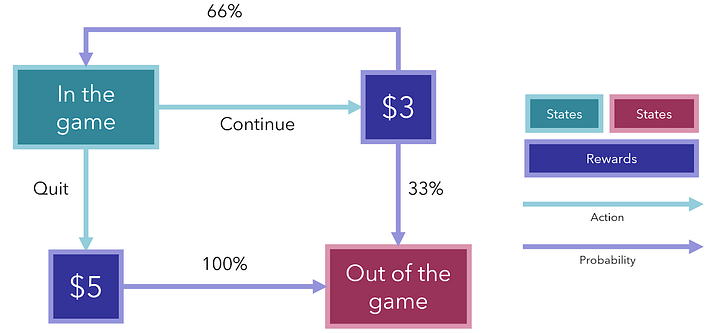
\includegraphics[scale=.4]{states}	
	\end{center}
\caption{Transition diagram}	
\end{figure}
\end{frame}	
\begin{frame}
\frametitle{Markov Decision Process}
\begin{block}{Definition}
	A \textbf{Markov Decision Process} is a $4$-tuple $(S, A_s, P_a, R_{s,a})$ where
	\begin{itemize}
		\item $S$ is a set, the set of states,
		\item $A$ is the set of actions (or $A_s$ actions available from state $A$).
		\item $P_a$ is the transition probability : prob. to move from one state to another after an action $a$.
		\item $R_{s,a}$ is the reward or penalty obtained after doing any move. 
	\end{itemize}
\end{block}
The goal of the decision-making is to maximize the reward by choosing the nicest actions.
\end{frame}
	\begin{frame}
	\frametitle{Markov Decision Process: Applications}

		 Markov Decision Process (MDP) is a type of Markov Chain model used in reinforcement learning.
		
		Some real-world example of MDP are:
	\begin{itemize}
		\item  robot navigation, where the agent has to navigate through an environment to reach a goal while avoiding obstacles.
		\item Automatic car control...
	\end{itemize}
\end{frame}
\section{Hidden Markov Model}
	\begin{frame}
		\frametitle{Hidden Markov Model}
		\begin{itemize}
			\item Hidden Markov Model (HMM) is a type of Markov Chain model widely used in speech recognition, image processing, and bioinformatics.
			\item HMM assumes that the observations are generated from a set of hidden states.
			\item A real-world example of HMM is speech recognition, where the hidden states are the phonemes and the observations are the audio signals.
		\end{itemize}
	\end{frame}
	

	\section{Reccurent Neural Network}
	\begin{frame}
		\frametitle{Recurrent Neural Network}
		\begin{itemize}
			\item Recurrent Neural Network (RNN) is a type of neural network that can capture sequential dependencies in data.
			\item RNN is a generalization of Markov Chain model that can capture long-term dependencies.
			\item A real-world example of RNN is natural language processing, where the model has to predict the next word in a sentence based on the previous words.
		\end{itemize}
	\end{frame}
	
	\begin{frame}
		\frametitle{Conclusion}
		\begin{itemize}
			\item Markov Chain models are versatile and powerful tools for modeling sequential data.
			\item They have a wide range of applications in various fields, including Machine Learning.
			\item In this presentation, we explored some real-world examples of Markov Chain models in Machine Learning.
		\end{itemize}
	\end{frame}
	
\end{document}